\chapter{Bridges, Cut Vertices, Cut Sets}

Remembering that he had not told Ajur about many concepts related to graph connectivity for both undirected and directed graphs, Rishnak went looking for Ajur. He found Ajur and Jura walking across a bridge that spanned a small brook.

Rishnak said, ``Today let us talk about graph connectivity.''

Ajur said, ``Okay, but already did, and I remember that for a graph to be connected, there has to be a path between every pair of vertices.''

Rishnak smiled and said that was correct. He continued, ``A \textit{bridge} is an edge in a connected graph that, when removed from that graph, causes the graph to become disconnected. Have a look at this graph''---Rishnak flashed his hands and a graph appeared in the air [Figure~\ref{14g1}]---``and you will find that every edge is bridge.''

Ajur said, ``I see. Every edge is a bridge because that graph is a tree.''

\begin{figure}
\begin{center}

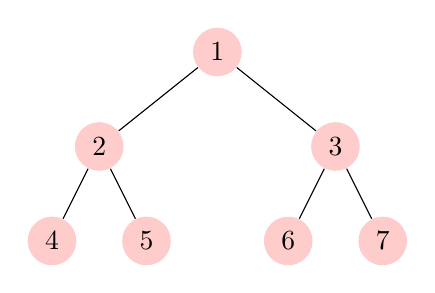
\begin{tikzpicture}
  [scale=.6,auto=left,every node/.style={circle,fill=red!20}]
  \node (n1) at (5.5,7) {1};
  \node (n2) at (3,5)  {2};
  \node (n3) at (8,5)  {3};
  \node (n4) at (2,3) {4};
  \node (n5) at (4,3)  {5};
  \node (n6) at (7,3)  {6};
  \node (n7) at (9,3)  {7};

  \foreach \from/\to in {n1/n2,n1/n3,n2/n4,n2/n5,n3/n6,n3/n7}
    \draw (\from) -- (\to);

\end{tikzpicture}
\caption{In a tree, every edge is a bridge}\label{14g1}
\end{center}
\end{figure}

Rishnak flashed his hands again and a second graph appeared [Figure~\ref{14g2}]. He said, ``And in this familiar graph, only one edge is a bridge.''

\begin{figure}
\begin{center}
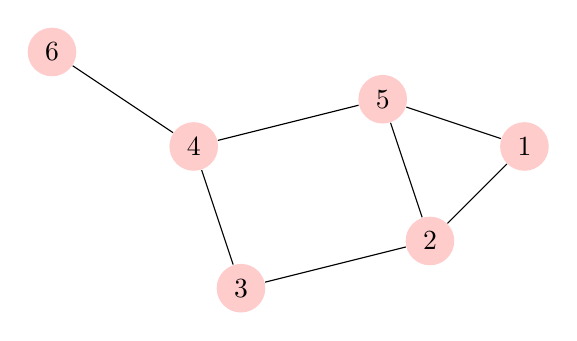
\begin{tikzpicture}
  [scale=.6,auto=left,every node/.style={circle,fill=red!20}]
  \node (n6) at (1,10) {6};
  \node (n4) at (4,8)  {4};
  \node (n5) at (8,9)  {5};
  \node (n1) at (11,8) {1};
  \node (n2) at (9,6)  {2};
  \node (n3) at (5,5)  {3};

  \foreach \from/\to in {n6/n4,n4/n5,n5/n1,n1/n2,n2/n5,n2/n3,n3/n4}
    \draw (\from) -- (\to);

\end{tikzpicture}
\caption{A graph in which only one edge is a bridge, i.e.,~removing edge~$(4,6)$ would cause the graph to be disconnected}\label{14g2}
\end{center}
\end{figure}

Rishnak said, ``A bridge is an important edge in a graph. As you have seen, if a bridge is removed---in other words, if that edge fails---then the graph becomes disconnected. It is certainly possible for a graph to not contain any bridges. For example, in a complete graph, there are no
bridges.''

Ajur asked Rishnak whether there was a concept similar to a bridge for vertices.

Rishnak said, ``Yes, a \textit{cut vertex} is a vertex that, when removed from a graph\footnote{Remember that removing a vertex means that all edges incident on that vertex are also removed from the graph.} causes the graph to be disconnected. In the second graph [Figure~\ref{14g2}], vertex~4 is a cut vertex.''

Ajur studied the graph and said, ``I see.''

Rishnak continued, ``And if you consider the map of the continental United States with states represented as vertices and borders defined by edges, New Hampshire is a cut vertex. If you remove New Hampshire from the graph, it is no longer possible to go from Maine to the other states. Similarly, in India, West Bengal is a cut vertex since its removal from the graph would cause northeastern states such as Assam to be no longer accessible from Kerala!''

Ajur thought for a moment, then said, ``In a tree, all vertices other than leaf vertices are cut vertices. And in a complete graph, there are no cut vertices. So if a graph has a cut vertex, that graph is vulnerable and may become disconnected if the cut vertex fails. Like a network with a single point of failure.''

Rishnak said, ``Precisely. And further, a graph is~$k$-connected if there is a set of~$k$ vertices that, when removed from the graph, causes the graph to become disconnected.''

Ajur realized that the concept of a graph being~$k$-connected was a generalization of a graph having a cut vertex since in that case,~$k=1$.

Rishnak continued, ``And similarly, a cut set is a set of edges that, when removed from the graph, causes it to be disconnected. How many vertices need to be removed from this graph''---Rishnak flashed his hands and a new graph appeared [Figure~\ref{14g3}]---``for it to become disconnected? And what is a cut set for this graph?''

\begin{figure}
\begin{center}

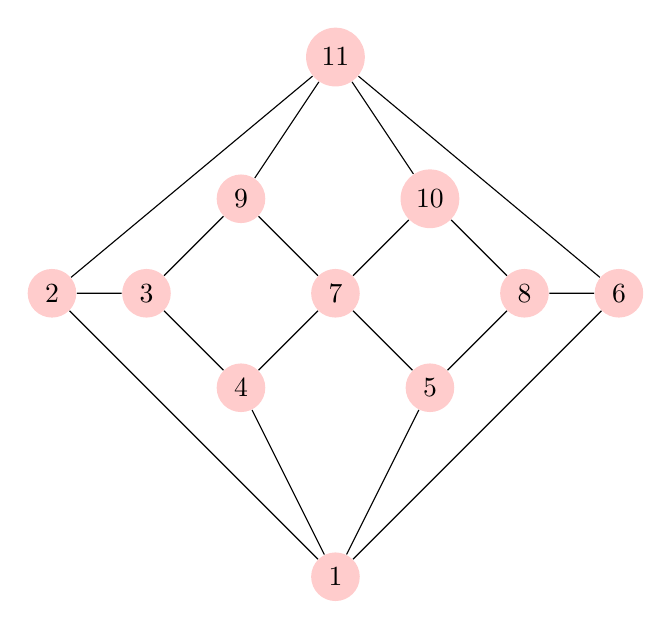
\begin{tikzpicture}
  [scale=.6,auto=left,every node/.style={circle,fill=red!20}]
  \node (n1) at (6,-3) {1};
  \node (n2) at (0,3)  {2};
  \node (n3) at (2,3)  {3};
  \node (n4) at (4,1) {4};
  \node (n5) at (8,1)  {5};
  \node (n6) at (12,3)  {6};
  \node (n7) at (6,3)  {7};
 \node (n8) at (10,3) {8};
  \node (n9) at (4,5)  {9};
  \node (n10) at (8,5)  {10};
  \node (n11) at (6,8)  {11}; 

  \foreach \from/\to in {n1/n2,n1/n4,n1/n5,n1/n6,n2/n3,n2/n11,n3/n4,n3/n9,n4/n7,n5/n7,n5/n8,n6/n8,n6/n11,n7/n9,n7/n10,n8/n10,n9/n11,n10/n11}
    \draw (\from) -- (\to);

\end{tikzpicture}
\caption{The old village road map of Royt for which we wish to determine how many vertices should be removed to cause the graph to be disconnected and also how many edges should be removed to cause the graph to be disconnected}\label{14g3}
\end{center}
\end{figure}

Ajur studied the graph and said, ``Removing vertices~1, 3, and~11 would cause the graph to be disconnected since that would isolate vertex~2. And similarly, a cut set is edges~$(2,1)$, $(2,3)$, and~$(2,1)$.''

\subsection*{Question for the twelfth day}
Rishnak said, ``Very good, Ajur.  Let us see now what the question is for the twelfth day. There are two parts to it. First, what is the largest number of bridges that a connected graph with~$n$ vertices, can have? And second, can you draw a graph with six vertices and exactly two bridges.?''

\textit{Before you turn the page, try to come up with answers of your own!}

\newpage
\subsection*{Answer for the twelfth day}
Ajur thought again about a tree, remembering that a tree is a minimally connected graph. He said, ``Since every edge in a tree is in a unique path, all of the edges of a tree are bridges. Therefore, the maximum number of bridges in a connected graph is~$n-1$ since this would be a tree of~$n$ vertices. And if we instead had~$n$ or more edges, then we would have a cycle, which means we would not be able to have the number of bridges be greater than or equal to~$n$.''

Rishnak nodded.

Ajur then grabbed a stick and drew a graph in the dirt [Figure~\ref{14ag1}]. He said, ``This graph has exactly six vertices and two bridges.''

\begin{figure}
\begin{center}
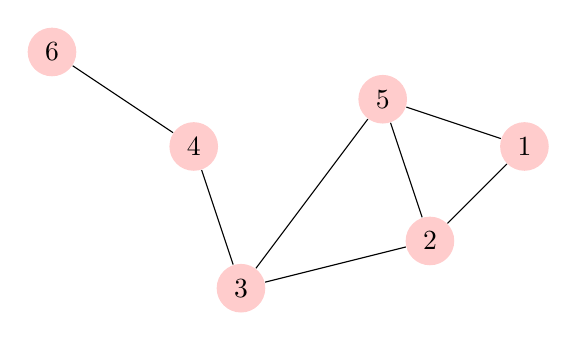
\begin{tikzpicture}
  [scale=.6,auto=left,every node/.style={circle,fill=red!20}]
  \node (n6) at (1,10) {6};
  \node (n4) at (4,8)  {4};
  \node (n5) at (8,9)  {5};
  \node (n1) at (11,8) {1};
  \node (n2) at (9,6)  {2};
  \node (n3) at (5,5)  {3};

  \foreach \from/\to in {n6/n4,n3/n5,n5/n1,n1/n2,n2/n5,n2/n3,n3/n4}
    \draw (\from) -- (\to);

\end{tikzpicture}
\caption{A graph with six vertices and two bridges, i.e.,~edges~$(6,4)$ and~$(4,3)$}\label{14ag1}
\end{center}
\end{figure}

Rishnak smiled and said, ``Good work, Ajur.''
